\chapter{NNQS deep dive}\label{nnqsresults}

In this chapter, we will explore the different architectures and training schemes that can be used for training the NNQS to solve QUBO problems.
\section{Comparing Architectures and training schemes}
We will compare the Restricted Boltzmann Machine (RBM) and the Multilayer Perceptron (MLP) in their performance as a NNQS. We will also compare 3 training schemes, namely direct, progressive, and continuous.

\subsection{NAE3SAT}
\begin{figure}[!h]
    \centering
    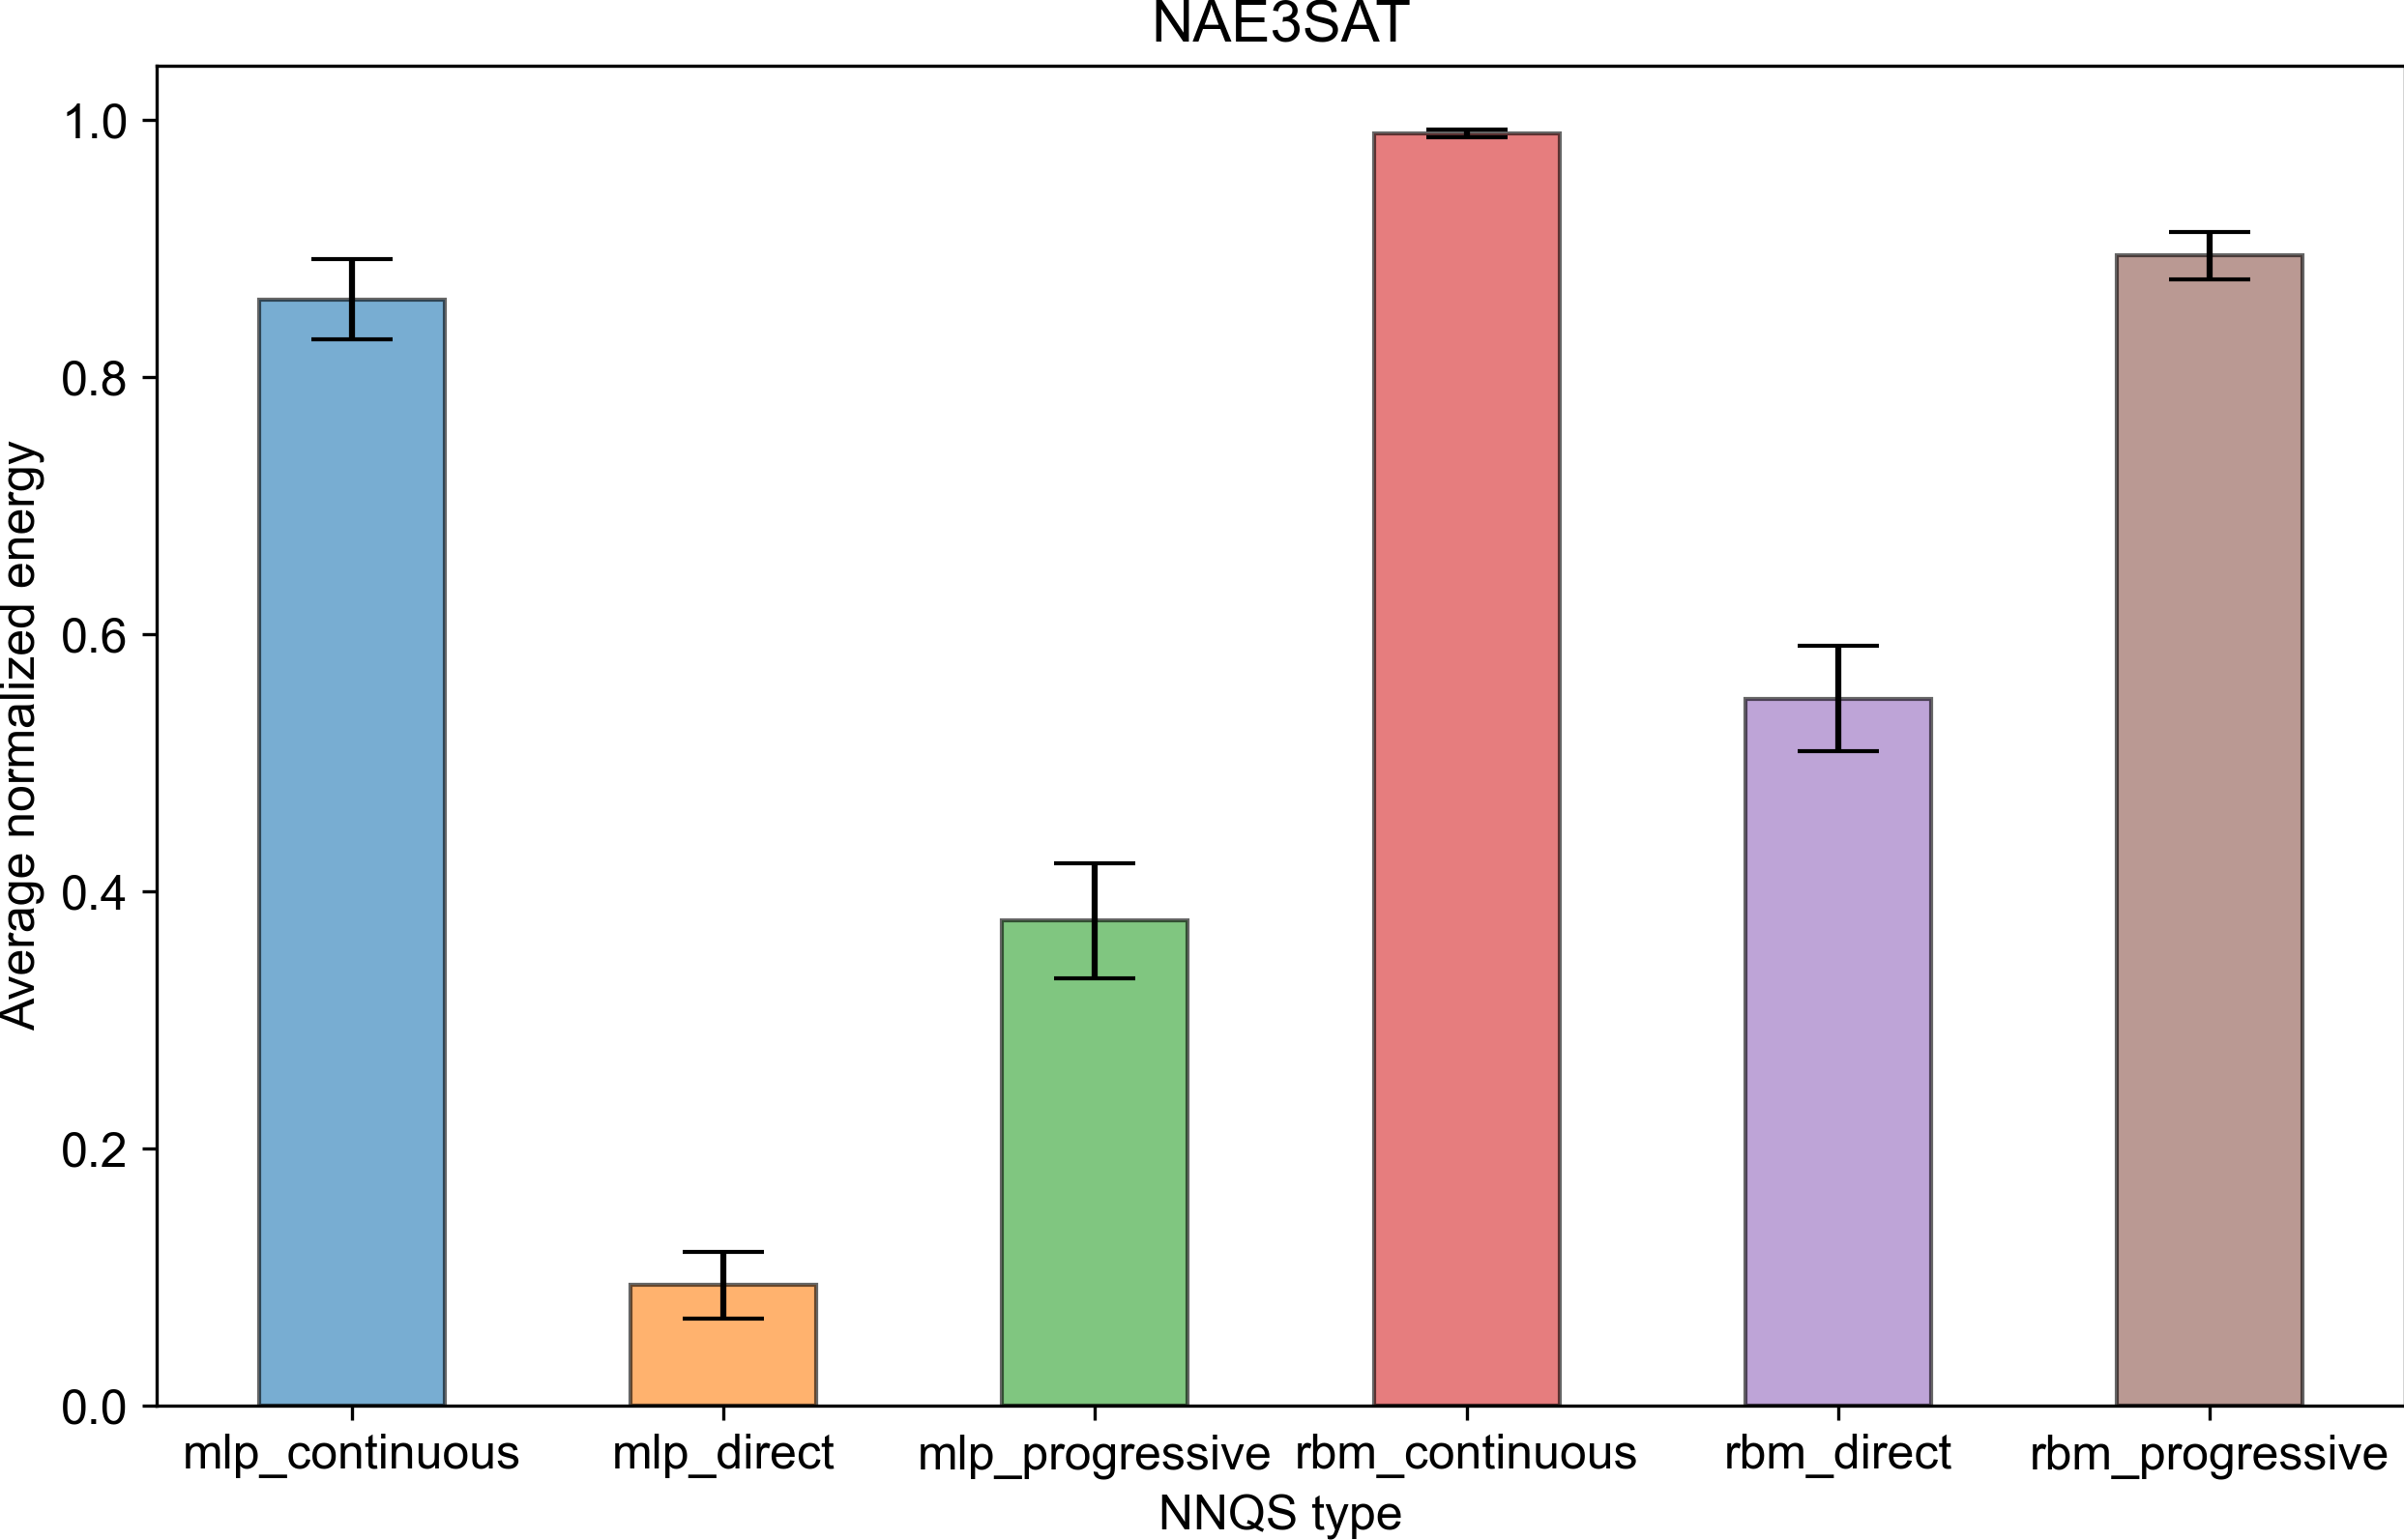
\includegraphics[width=1\linewidth]{images/nae3sat_nnqs_avg.png}
    \caption{Performance of different NNQS types on the NAE3SAT dataset}
    \label{nnqs-nae3sat-average}
\end{figure}

\begin{figure}[!h]
    \centering
    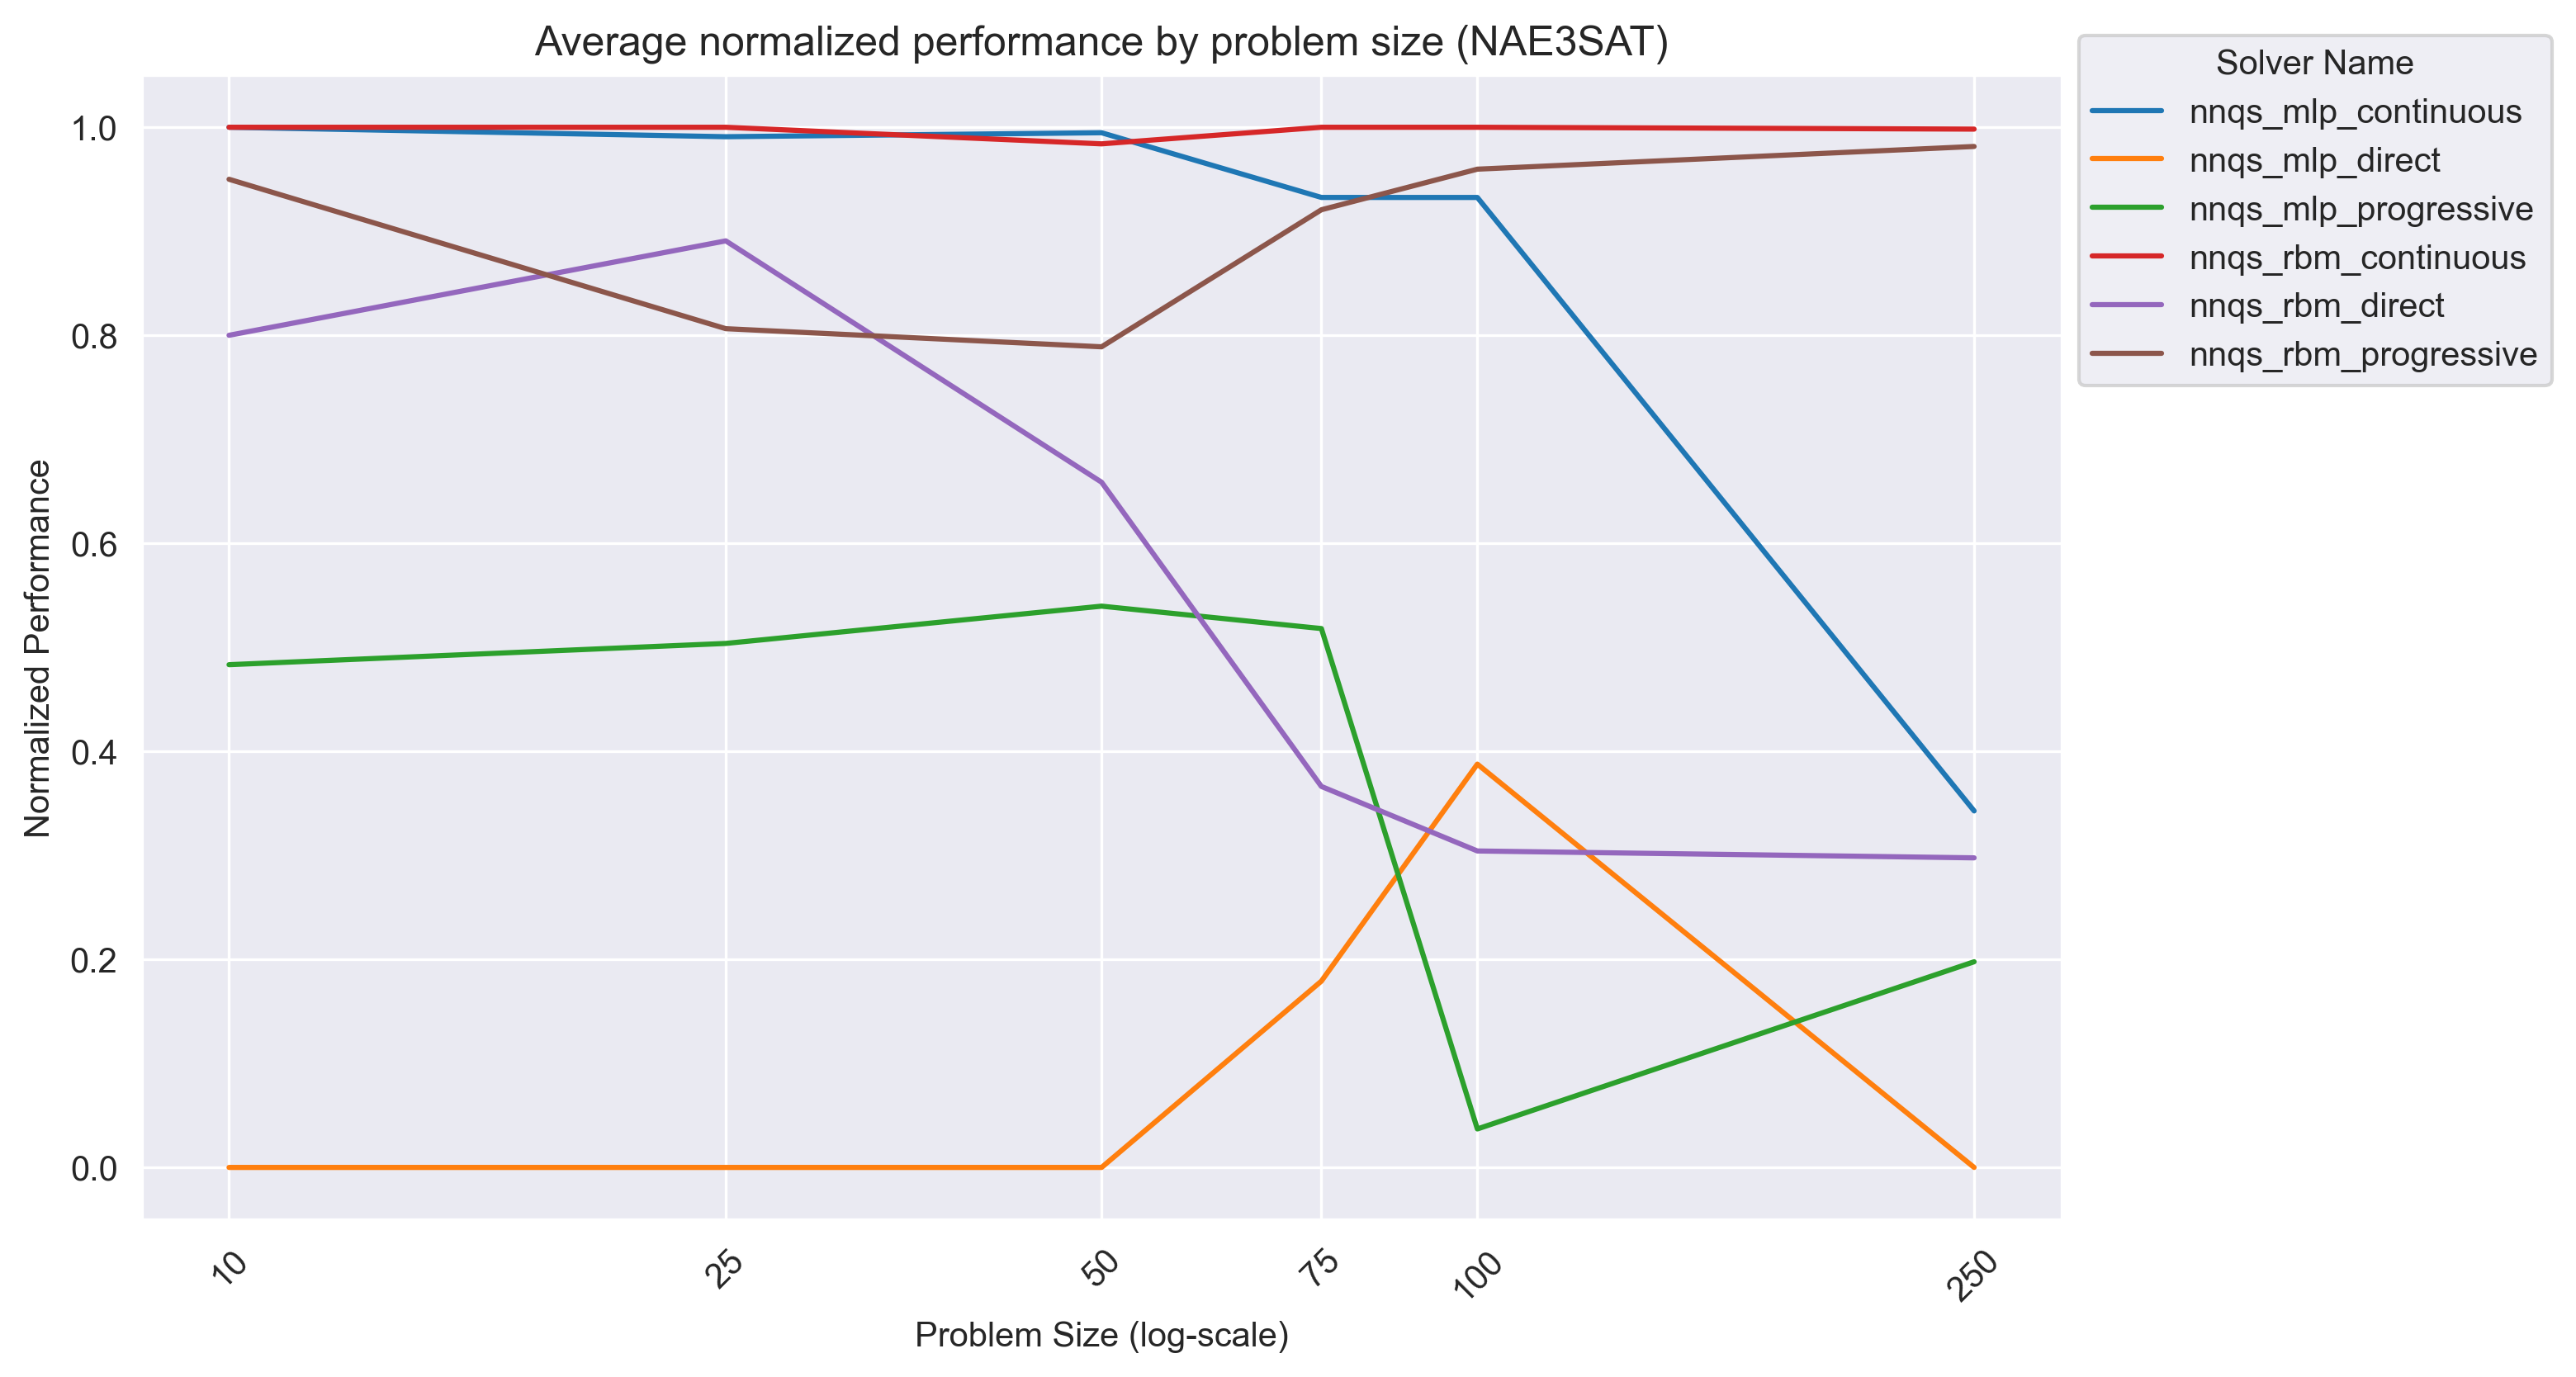
\includegraphics[width=1\linewidth]{images/nae3sat_nnqs_size.png}
    \caption{Performance by size on the NAE3SAT dataset}
    \label{nnqs-nae3sat-size}
\end{figure}

\subsection{Max-cut}
\begin{figure}[!h]
    \centering
    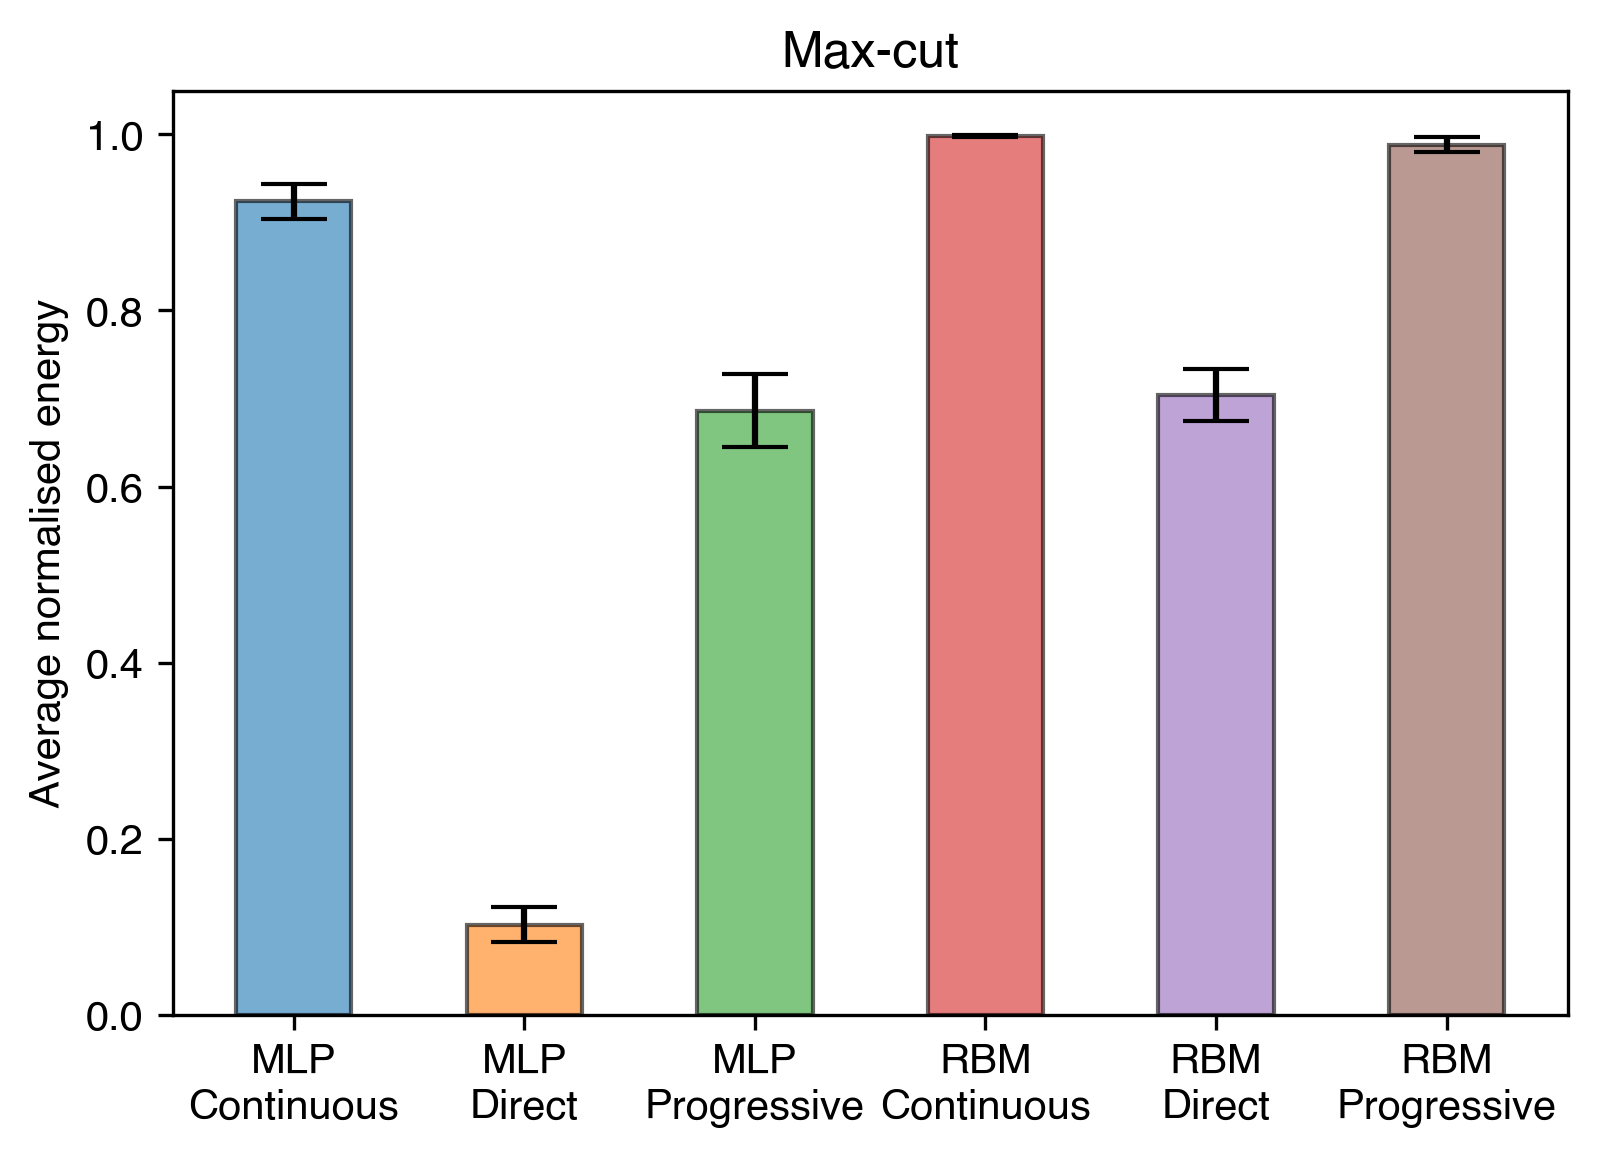
\includegraphics[width=1\linewidth]{images/maxcut_nnqs_avg.png}
    \caption{Performance of different NNQS types on the max-cut dataset}
    \label{nnqs-maxcut-average}
\end{figure}

\begin{figure}[!h]
    \centering
    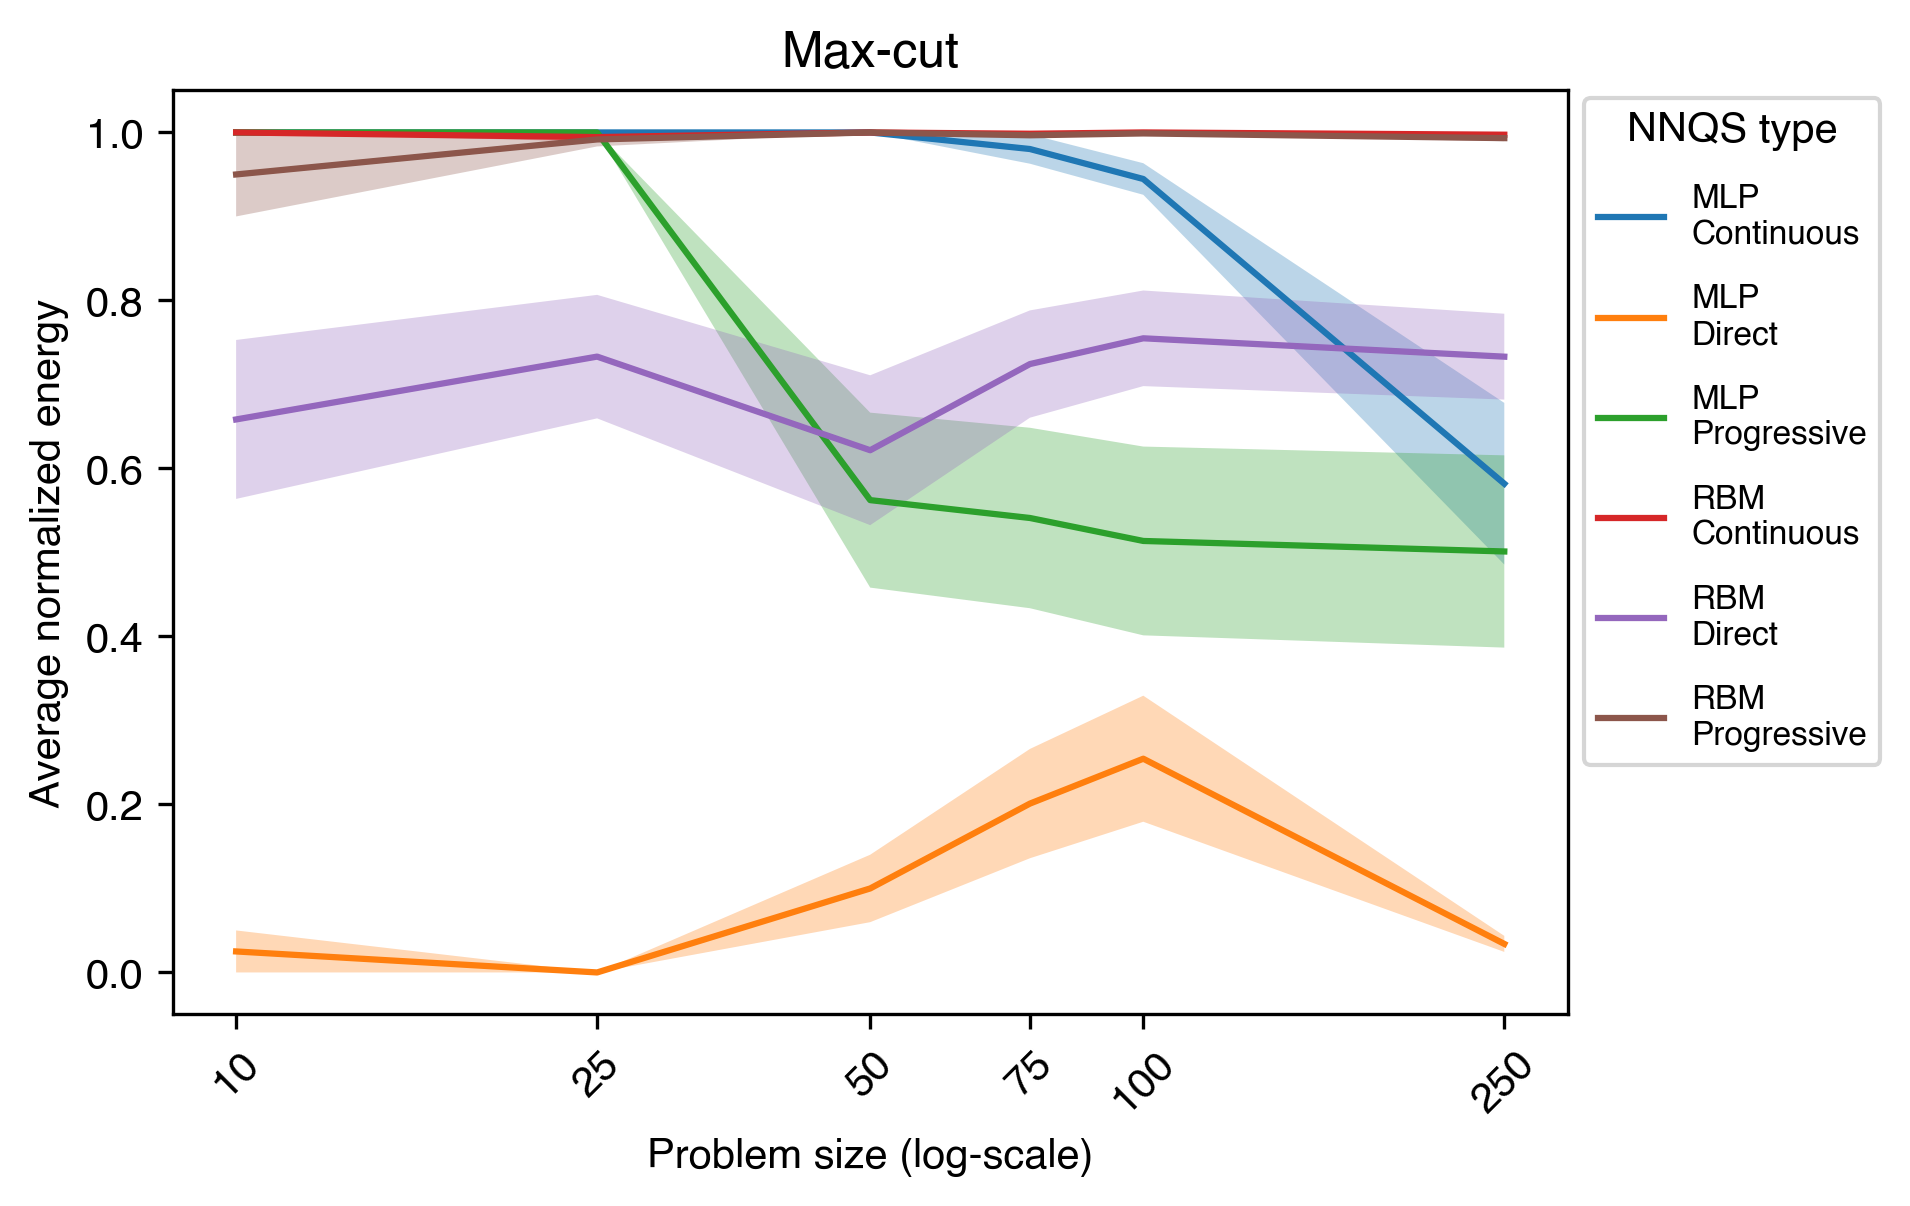
\includegraphics[width=1\linewidth]{images/maxcut_nnqs_size.png}
    \caption{Performance by size on the max-cut dataset}
    \label{nnqs-maxcut-size}
\end{figure}

\subsection{SK Model}
\begin{figure}[!h]
    \centering
    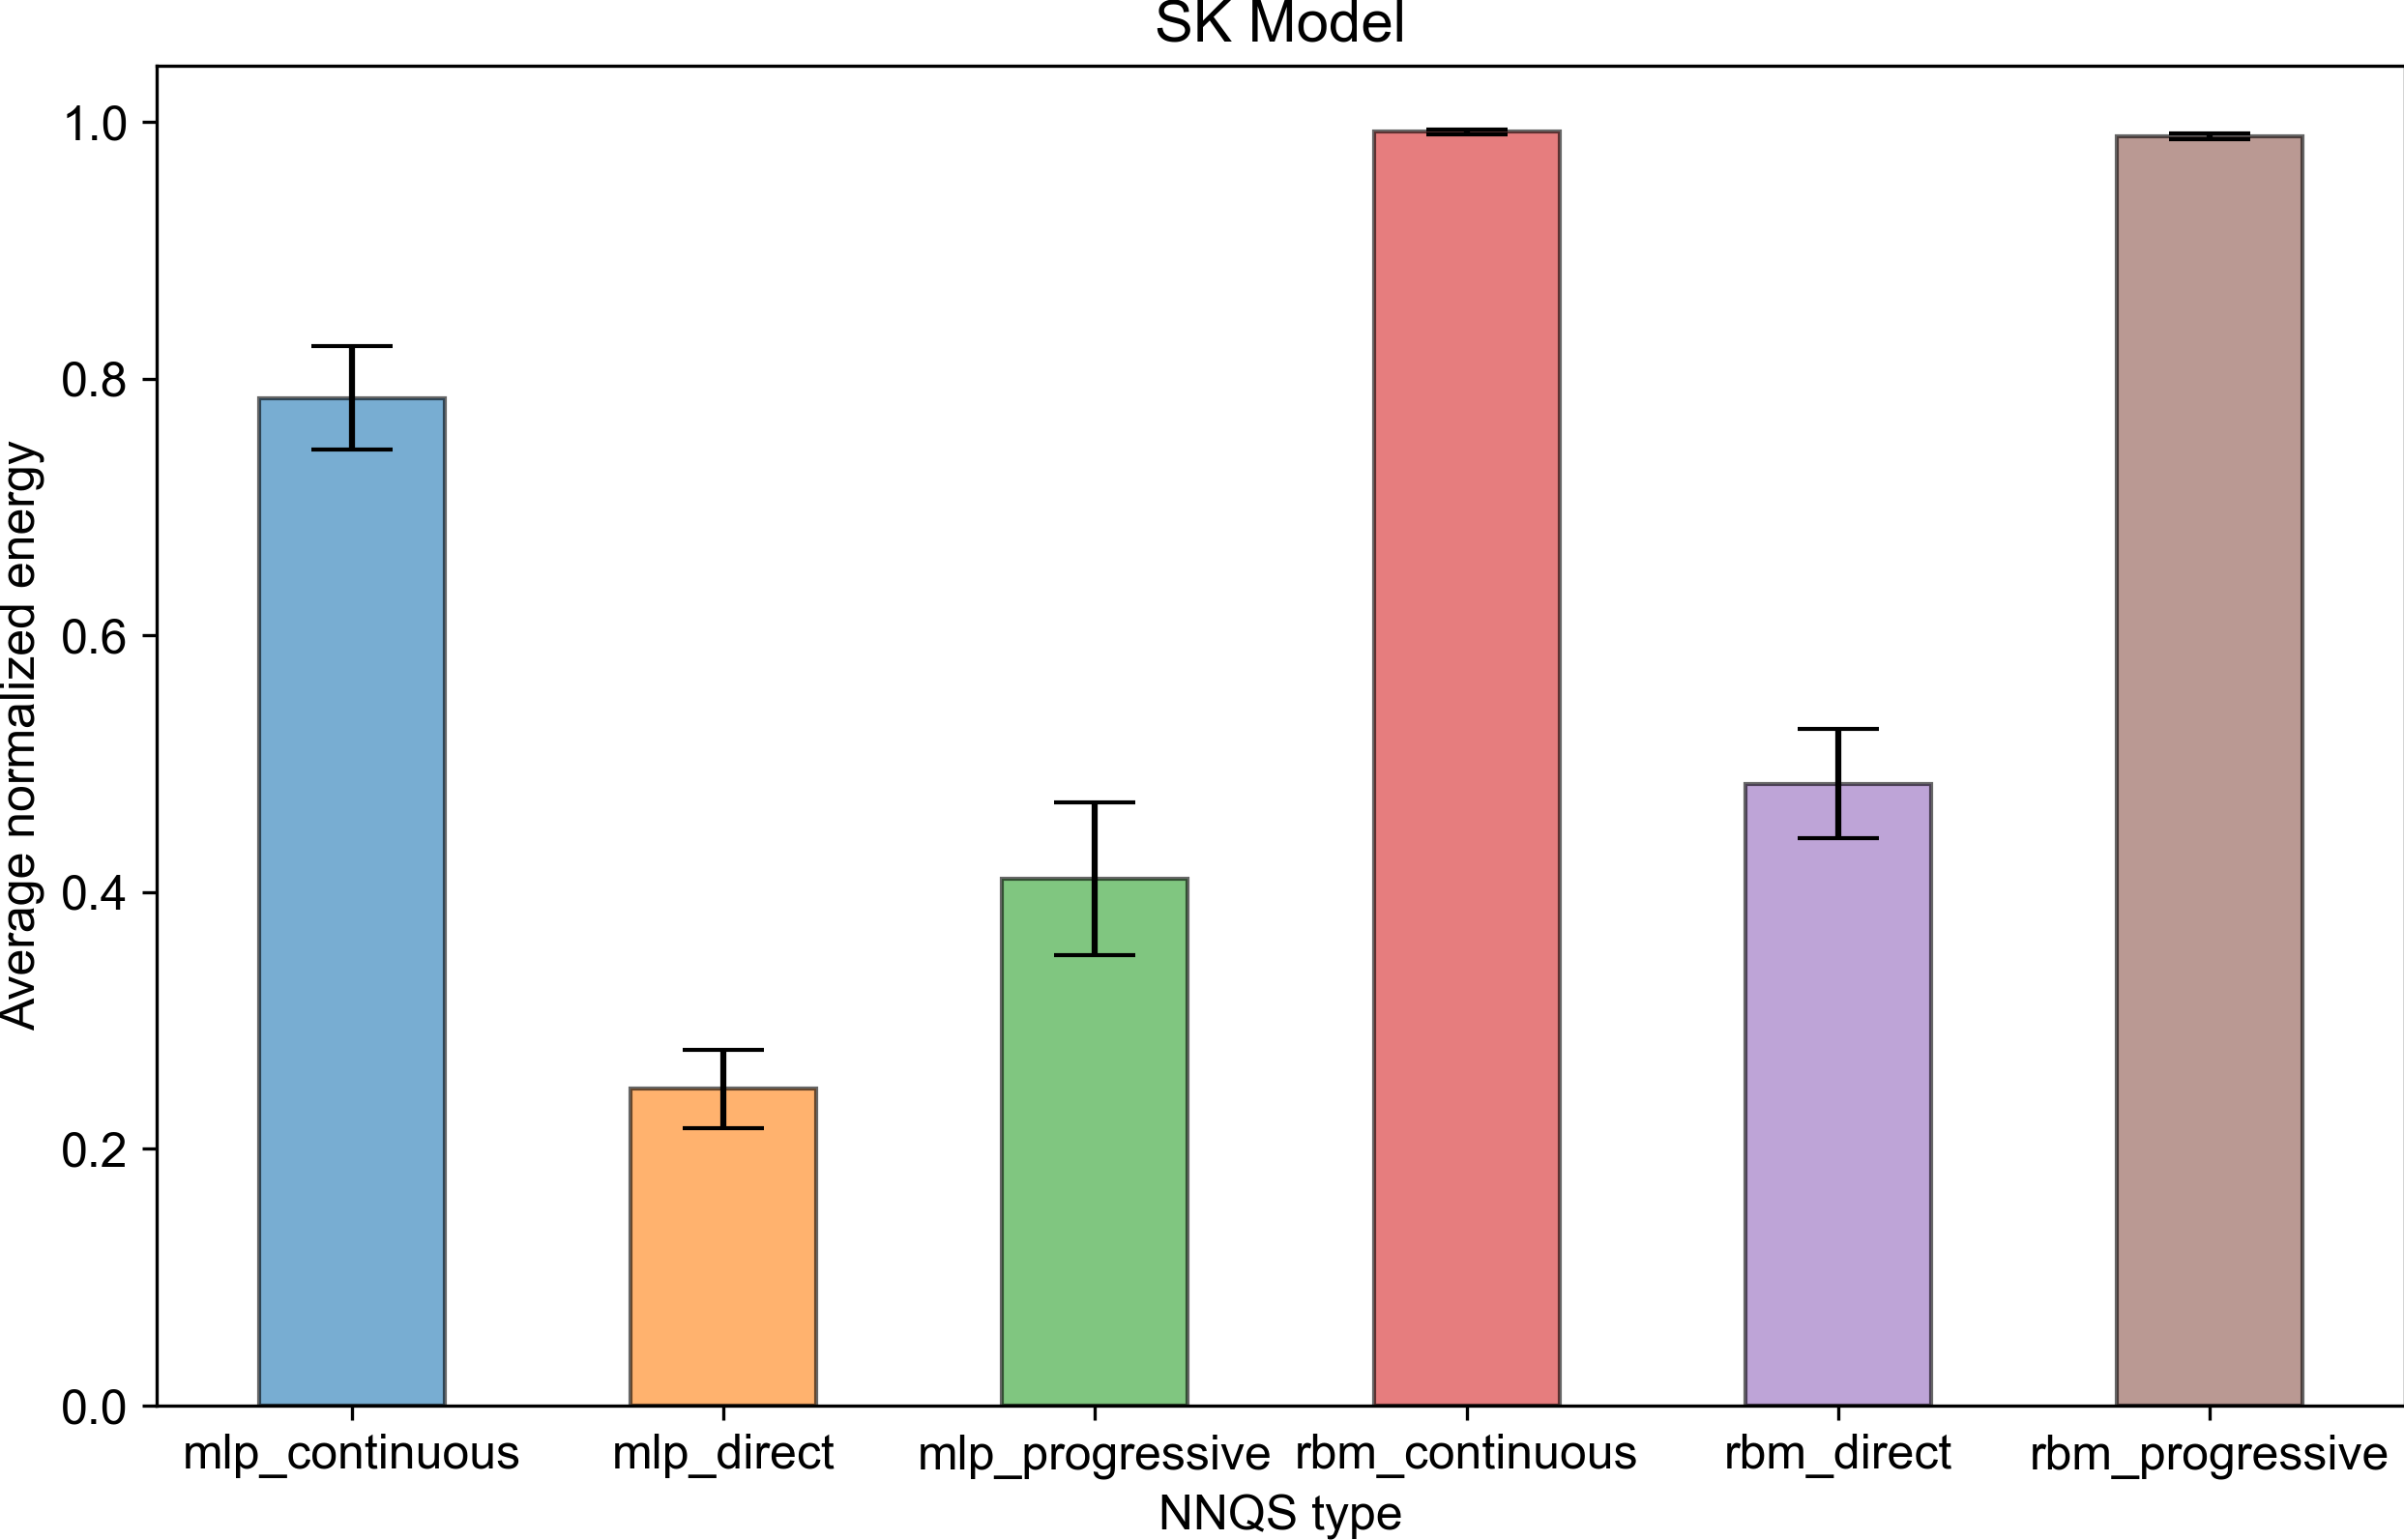
\includegraphics[width=1\linewidth]{images/skmodel_nnqs_avg.png}
    \caption{Performance of different NNQS types on the SK model dataset}
    \label{nnqs-skmodel-average}
\end{figure}

\begin{figure}[!h]
    \centering
    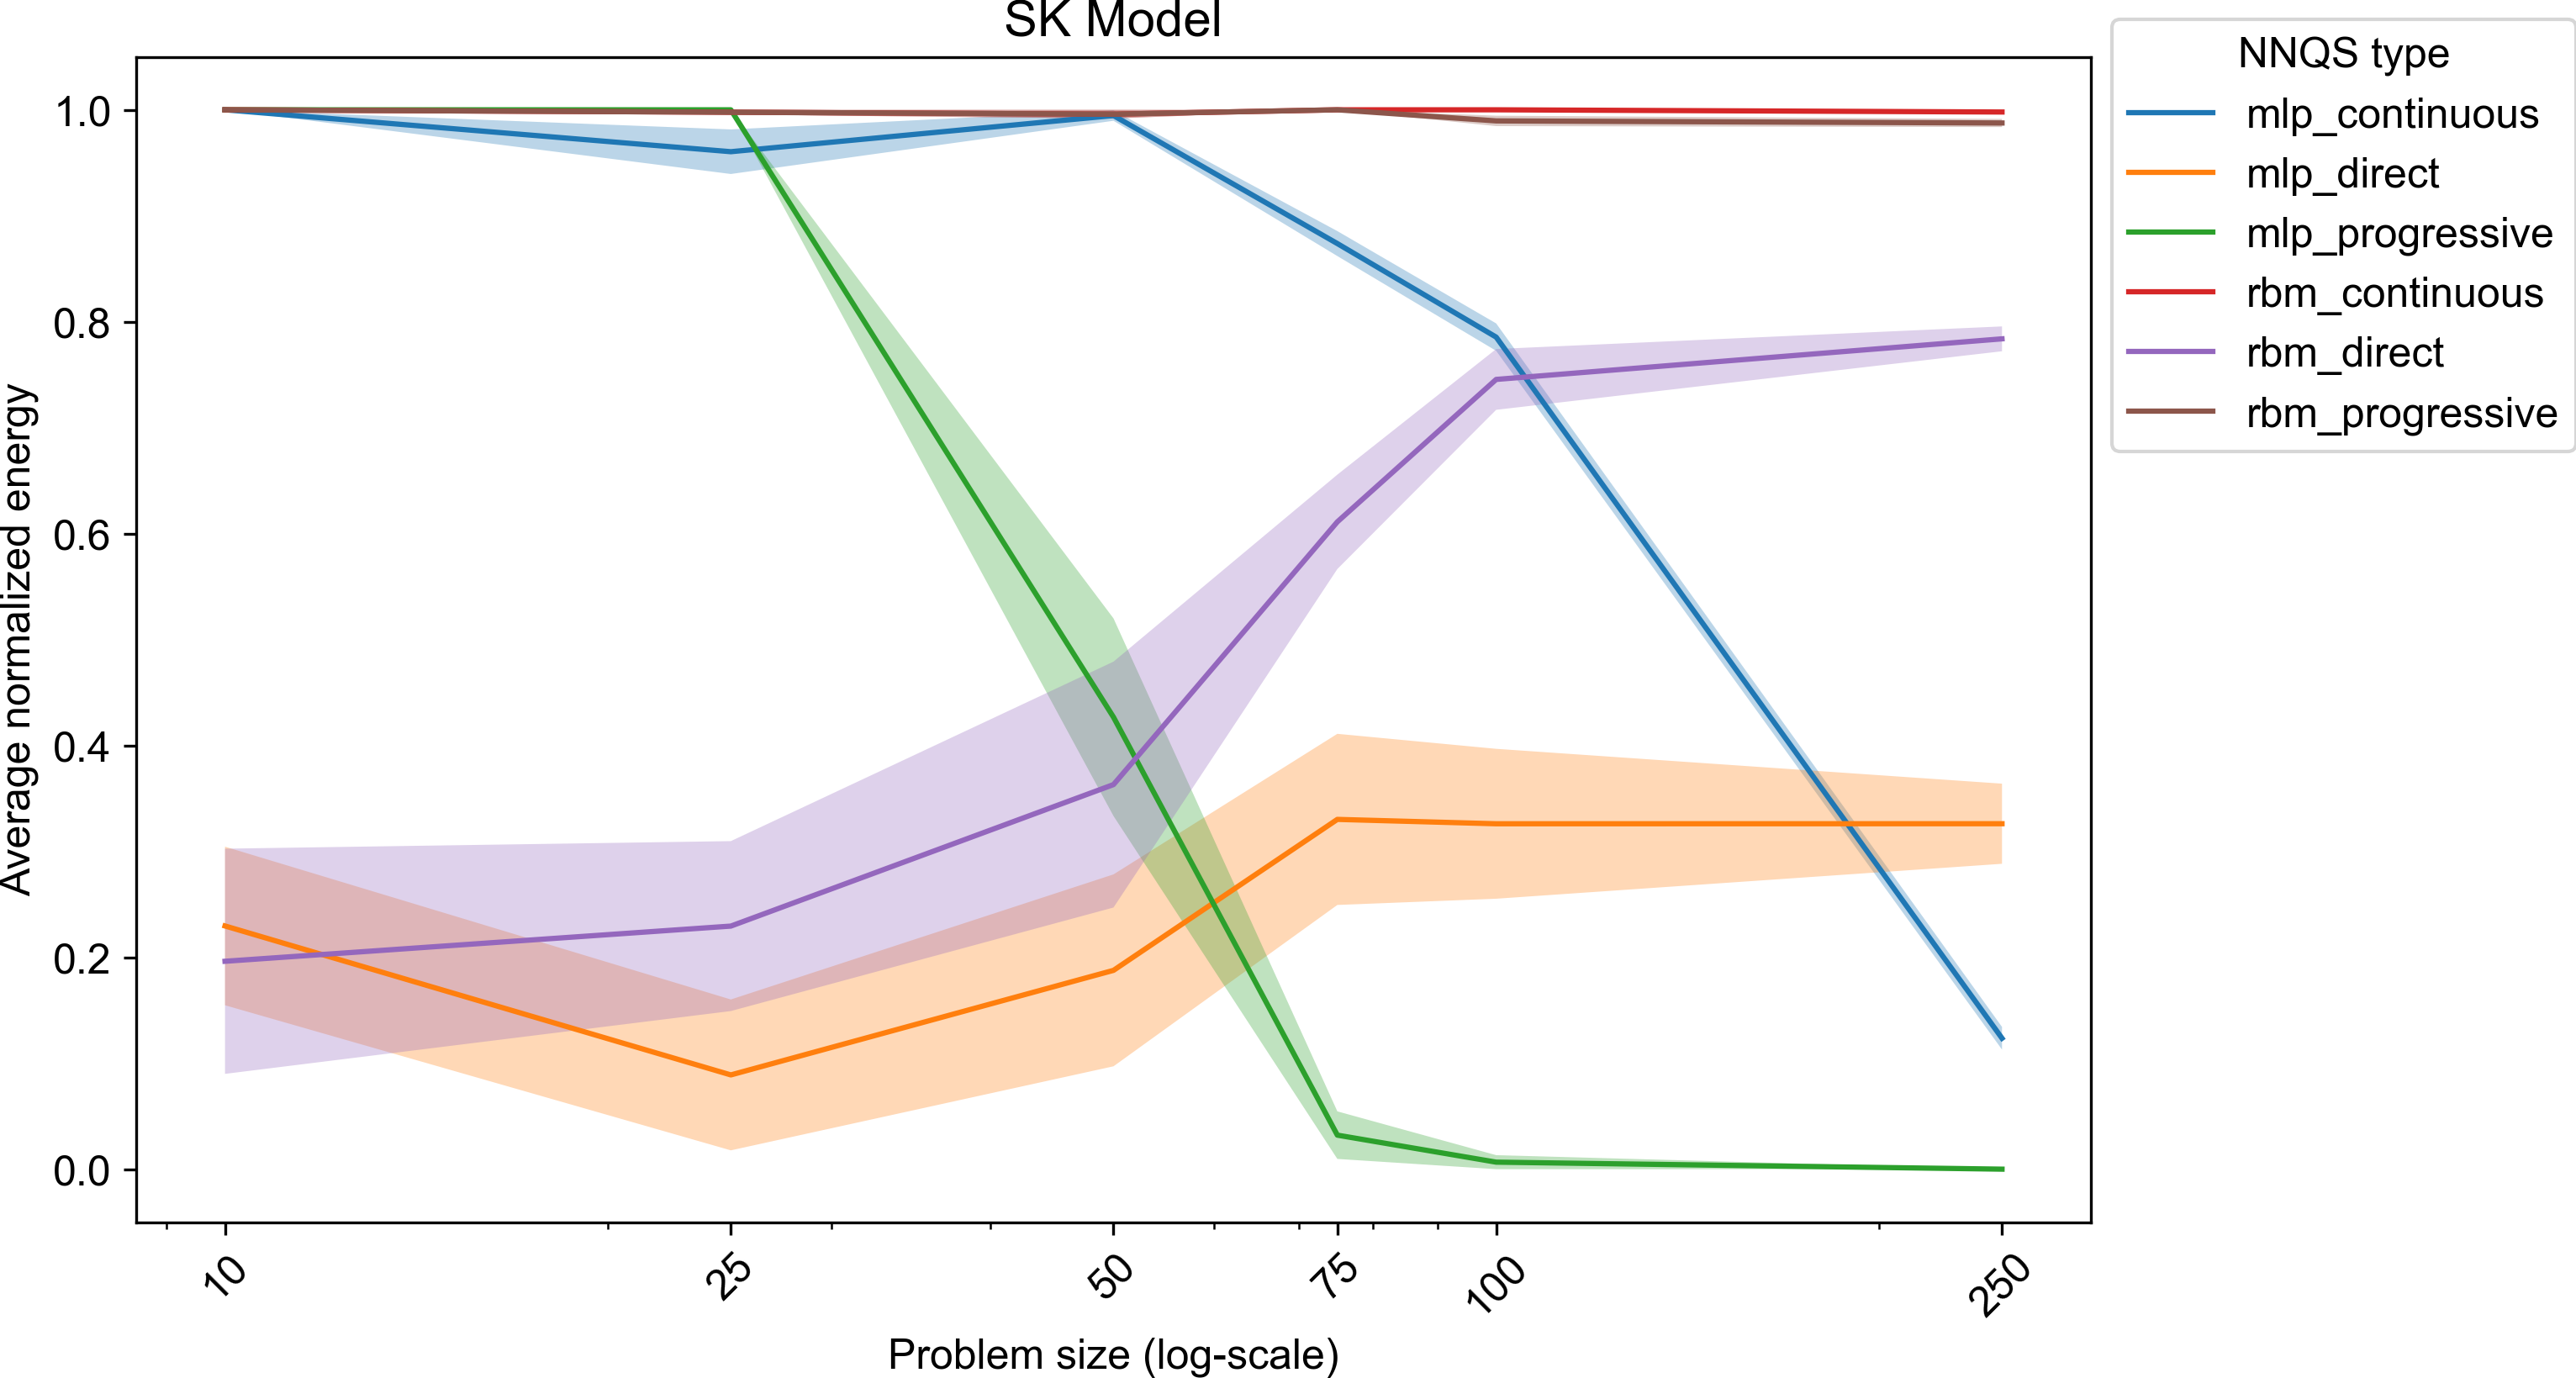
\includegraphics[width=1\linewidth]{images/skmodel_nnqs_size.png}
    \caption{Performance by size on the SK model dataset}
    \label{nnqs-skmodel-size}
\end{figure}

Using the RBM with a continuous training scheme gives the highest normalized performance across all datasets.

\section{Quenching}